\documentclass[a4paper,12pt,twocolumn]{article}
\usepackage[utf8]{inputenc}
\usepackage{graphicx}
\usepackage{hyperref}
\usepackage[toc,page]{appendix}
\usepackage{comment}

\title{
    Intelligent Control and Cognitive Systems\\
    \begin{large}
        Coursework 1 Report
    \end{large}
}
\author{Adam Jaamour & Tom Slattery}
\date{28th February 2019}

\begin{document}
\maketitle
\thispagestyle{empty}
\clearpage
\setcounter{page}{1}

% ----------------------------------------------------------------------------

\section{Introduction}

This experiment determines the effect of distance from the walls on the path taken of a wall following rover created with the LEGO Mindstorm EV3 kit.\\

The rover built in Figure \ref{fig:robot-portrait} uses a combination of touch sensors and a rotating ultrasonic sensor to detect its position in relation to the environment. A pair of servo motors allow the rover to navigate its environment. An "arena" was created of completely enclosing right-angled walls. A variety of combinations of concave and convex corners provide a challenging path for the rover to traverse.

\begin{figure}[ht]
\centering
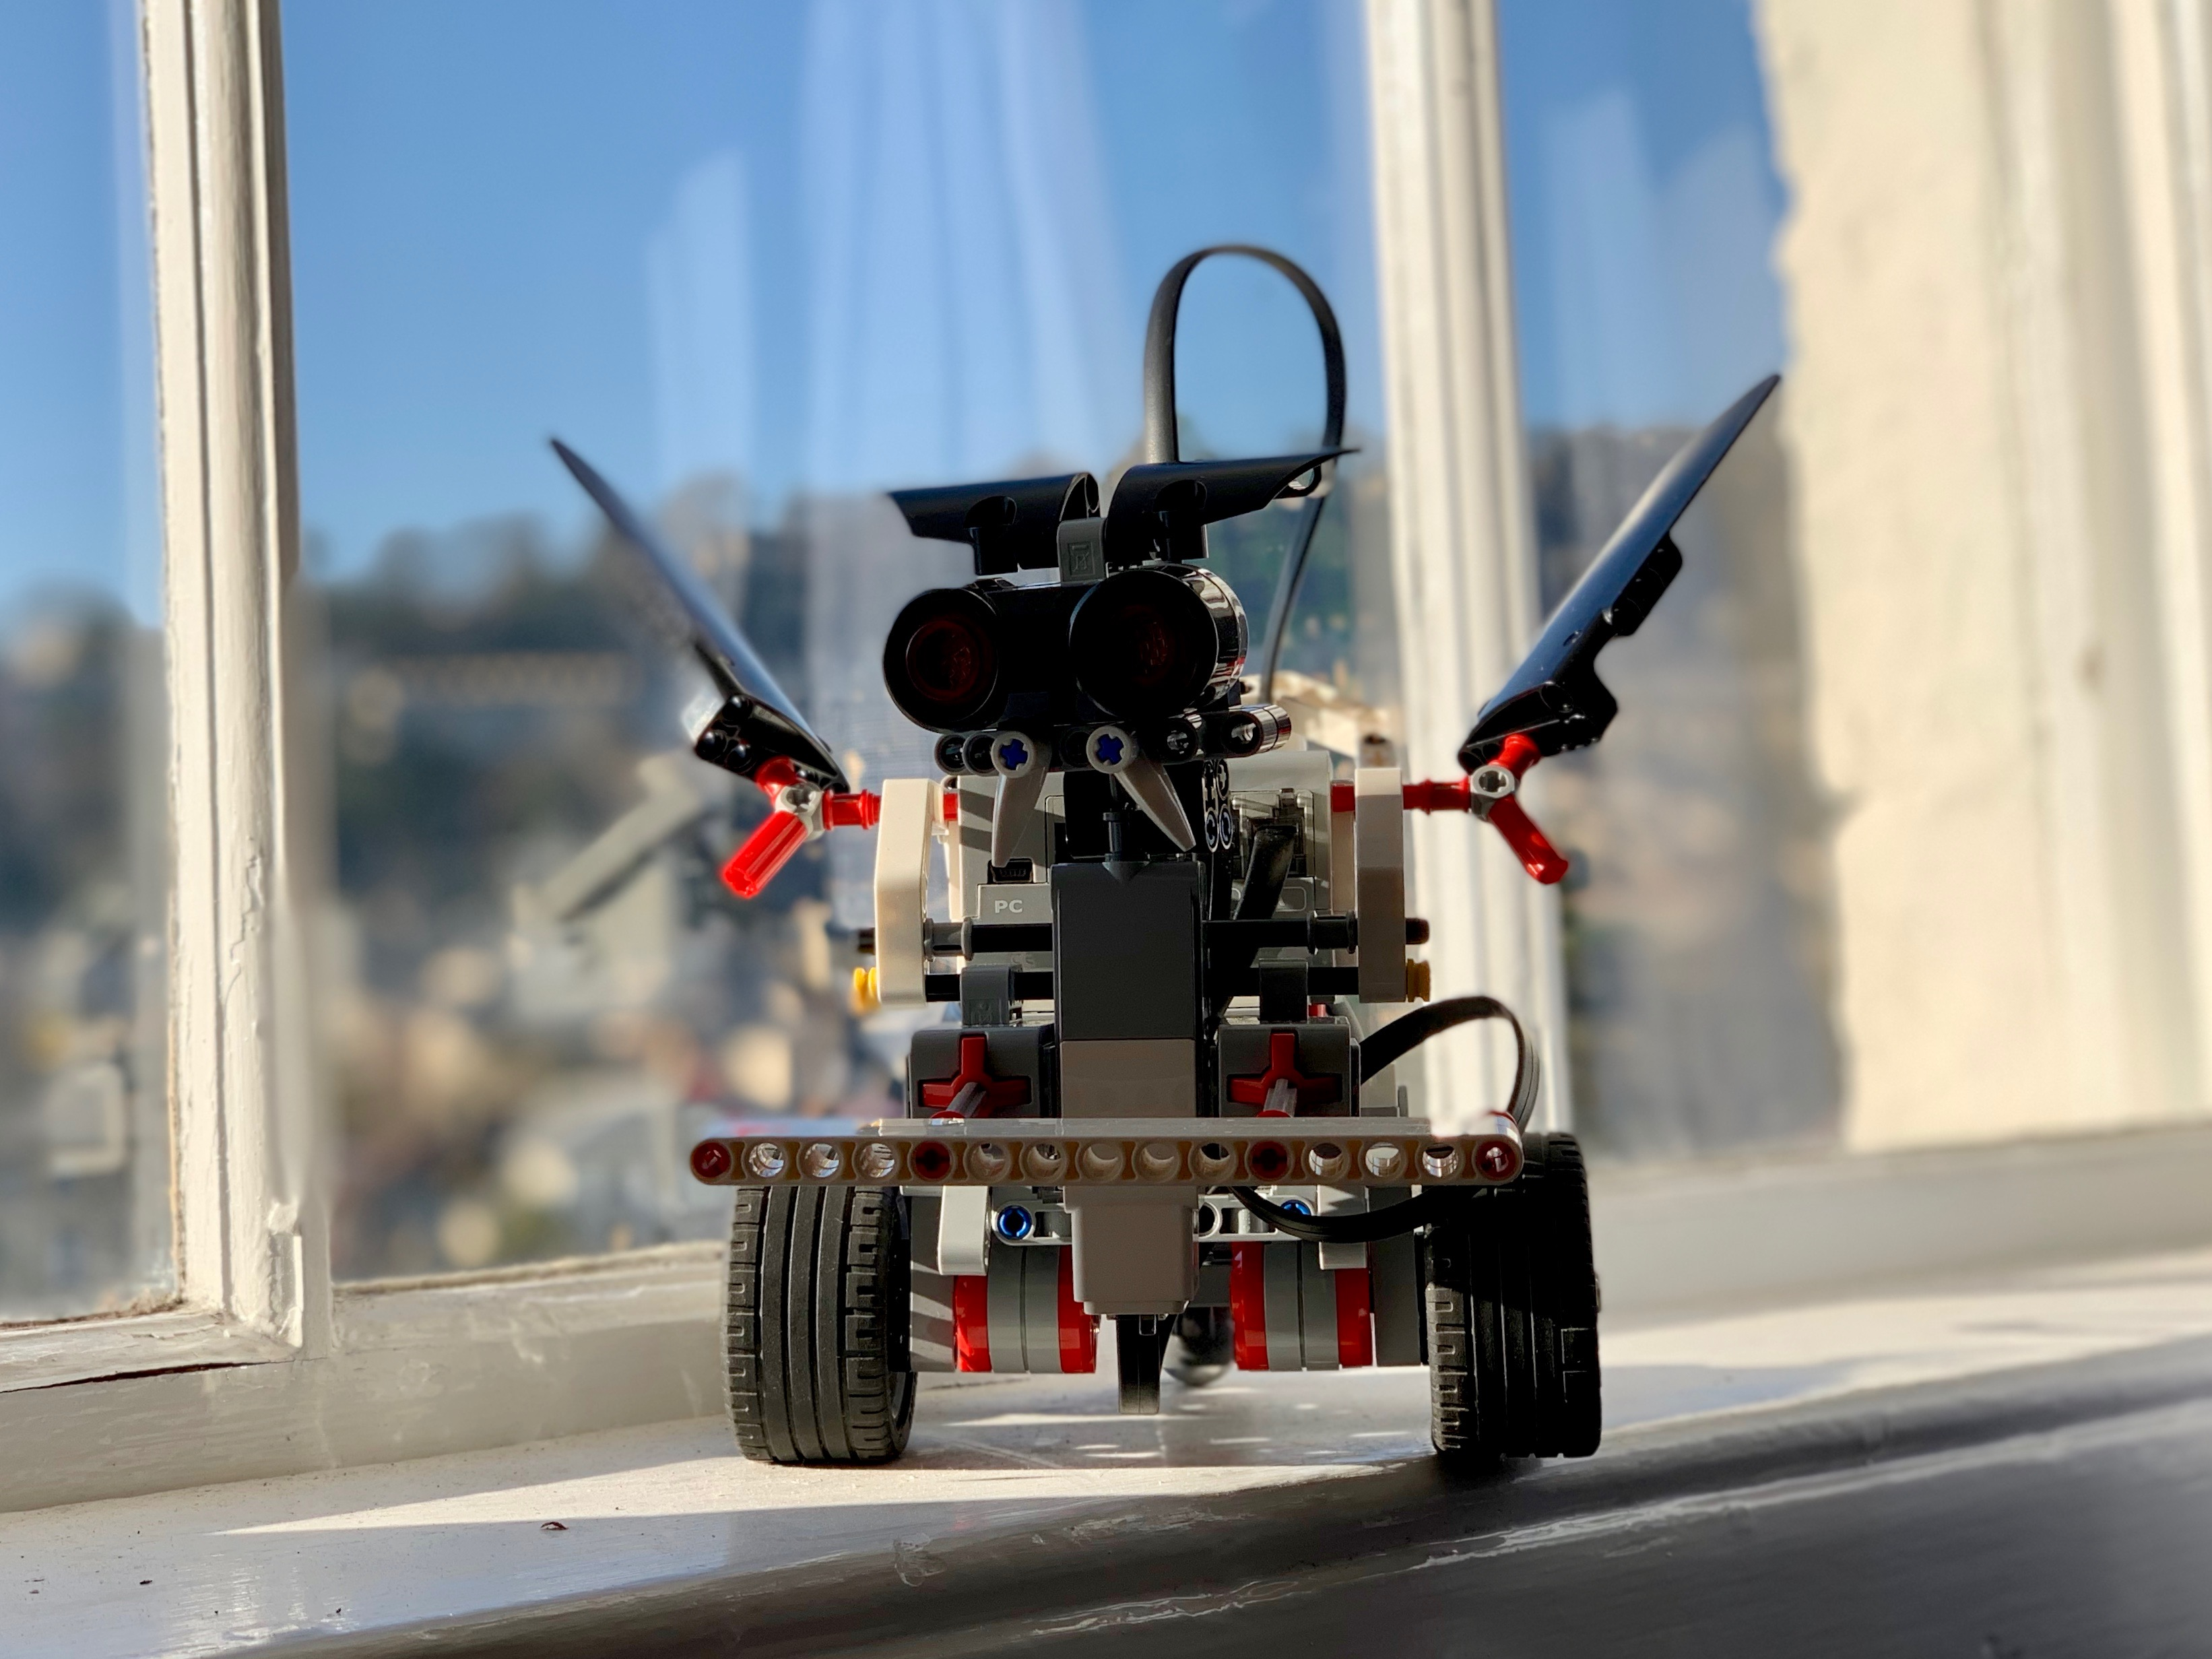
\includegraphics[width=\linewidth]{figures/robot_portrait.jpeg}
\caption{Robot portrait}
  \label{fig:robot-portrait}
\end{figure}

The following distance is related to both the time taken to traverse a given area and the number of collisions with the walls. It also directly effects the level of granularity with which the rover explores the more detailed parts of the enclosed area. The optimum following distance was found while maintaining a good level of coverage of the arena.\\

The rover is inspired by subsumption architecture, with the "end goal" of traversing the entire enclosure being split into sub-goals, including calculating the correct direction to turn using sensor data and remaining a fixed distance from the walls. However, this architecture would require a parallel implementation. A simple reflex agent model was applied instead, with a series wall following algorithm consisting of three states. This proved sufficient to traverse the arena easily and test the hypothesis. \\

The system software was created in Java, with source control using GitHub. 
 
\begin{comment}
Todo:
\begin{itemize}
    \item state goal of research
    \item state the different types of sensors used, design reasons (positioning of the sensors for better/optimal readings)
    \item include picture of the robot?
    \item specify approaches using references
    \begin{itemize}
        \item reactive approach using subsumption architecture (Wooldridge, 2009)
        \item --> to allow rover to determine its current situation
        \item using subsumption based on (Brooks, 1991) thesis
    \end{itemize}
\end{itemize}
\end{comment}

% ----------------------------------------------------------------------------

\section{Approach}
The EV3 rover was designed following the simple reflex agent architecture  \cite{brooks1991intelligence}\\

Two types of sensors are used to allow the rover to collect data about the environment. A pair of EV3 Touch Sensors are mounted on the front of the rover. They are responsible for detecting collisions with walls. A bar connects the two sensors for rigidity, with a collision being detected as a response from either sensor. This proved to make collision detection more reliable, as collisions at an angle were frequently ignored by a single touch sensor due to flexibility of the plastic Lego components. The bar also allowed a wider area in which collisions could be detected, meaning that direct collisions with an convex corner stops the rover before it becomes too close for the depth sensor to reliably function.\\

An Ultrasonic depth sensor is mounted on a rotating servo motor at the front of the rover. This is used in the "searching" state, once the touch sensors have been triggered. Due to the high noise floor of the readings from this sensor, an average of multiple readings is taken each time the sensor is used. The mean and standard deviation is found, and and any readings outside of a range of +/-1 * standard deviation are removed from the average.\\

Initial trials of the turning functions proved that the number of degrees rotated by the wheel motors did not correspond to the same rotation of the robot. The motors now compensate for factors such as turning friction by turning more than the desired angle, allowing the rover a more accurate rotation. \\

The rover software has three main states which can be transitioned between:
\begin{itemize}
    \item Initial State
    \item Searching
    \item Wall Following
\end{itemize}

The rover begins in the "initial state", travelling forwards until it hits a wall (as detected by the touch sensor). Once a wall is detected, the rover enters the "searching state". The possible configurations of the position of the robot in relation to the arena walls have been simplified to situations observable by the Ultrasonic sensor sweeping to the left and right.(Figure XXXXXXXXXXXXX).\\

The robot then turns by 90 degrees and rotates the ultrasonic sensor to face the wall. 
To ensure that the robot makes a full circuit of the arena, it is programmed to always make a right turn if it is possible to do so.\\

The rover then enters the "wall following state", and begins moving parallel to the wall. The ultrasonic sensor is used to maintain a constant distance. The distance from the wall is a controlled by a variable. The rover continues in this state until the touch sensors are triggered again.\\

The flow of control between these three states is detailed in the flowchart diagram in Figure \ref{fig:flowchart}.

\subsection{Experimental Procedure}

The rover is placed in an arena, consisting of fully enclosing right angled walls depicted in Figure \ref{fig:arena-layout}. The robot begins from a designated starting line. The shape of the arena is preserved between trials.\\

\begin{figure}[ht]
\centering
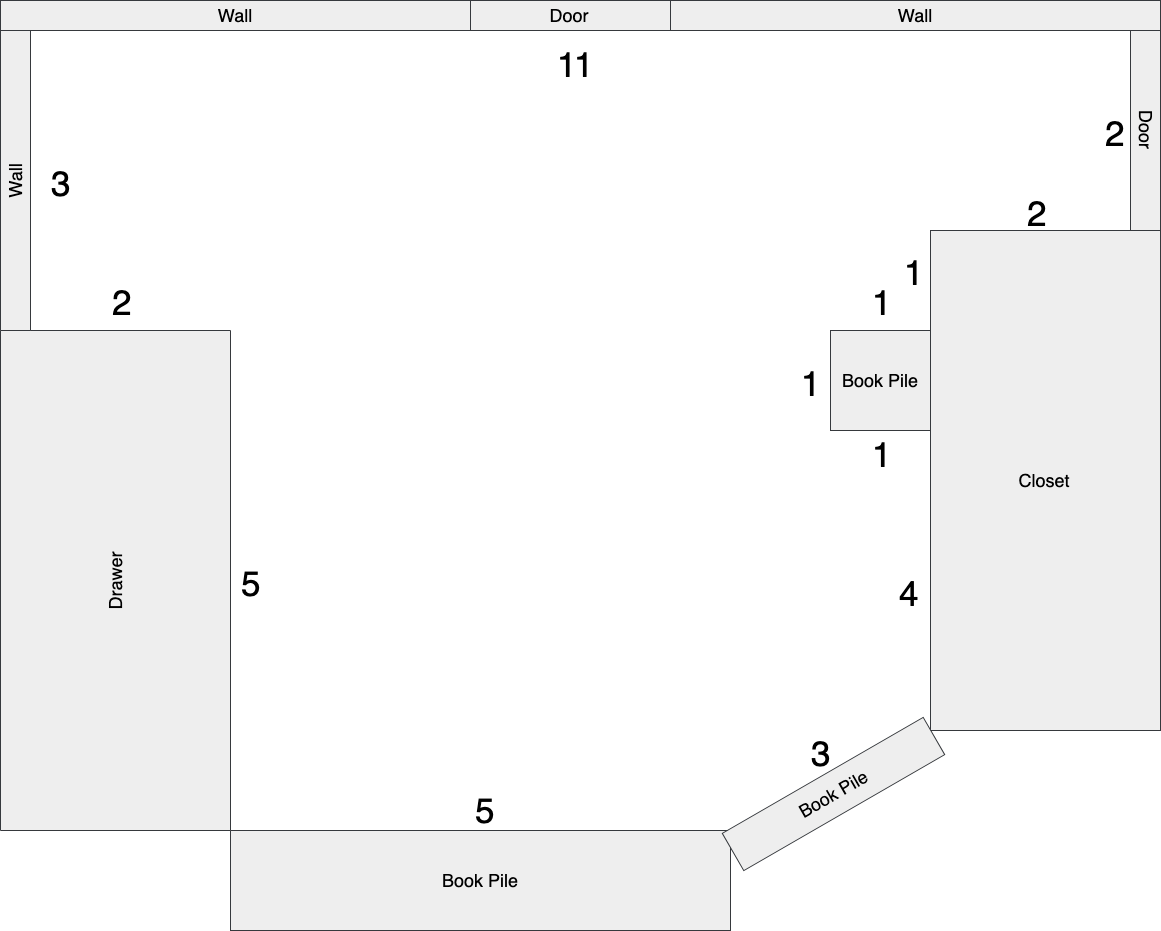
\includegraphics[width=\linewidth]{figures/arena-layout/Arena Layout.png}
\caption{Arena layout}
  \label{fig:arena-layout}
\end{figure}

A single trial consists of one full lap of the arena, returning to the starting point. The distance maintained from the wall during the wall following state is controlled as an independent variable. The time taken to traverse back to the starting point and the number of wall collisions are dependent variables which are recorded during each trial. Two trials are performed for each distance.\\

If the rover becomes stuck or pushes a wall the trial is aborted.  

\begin{comment}
Todo:
\begin{itemize}
    \item initial design of rover is usually a simple reflex agent (Russell et al., 1995), allows rover to react to state CRASH but no context for recovery is provided
    \item final design: model-based reflex agent (Russell et al., 1995) allows sensors to modify state
    \item include a perception architecture figure?
    \item describe rover rates of measurements per second
    \item end by formulating hypothesis e.g. "the rover will perform better if threshold is higher, or if measurements per second is higher, or if 
    \item figure showing layout of the track/obstacles?
    \item mention who did what in the rover's design
    \item mention how morphology helps (wings can help it turn in corners)
\end{itemize}
\end{comment}

\begin{figure*}[ht]
\centering
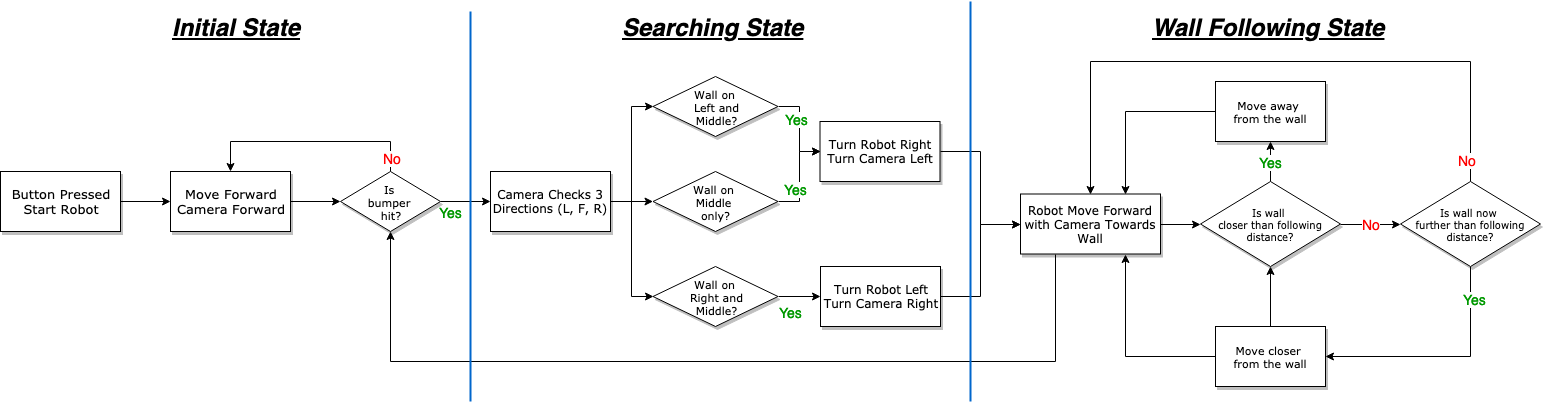
\includegraphics[width=\linewidth]{figures/flowchart/System-Flowchart.png}
\caption{Flowchart}
  \label{fig:flowchart}
\end{figure*}

% ----------------------------------------------------------------------------

\section{Results}
Three hypotheses were tested by the experiment:
\begin{itemize}
    \item Maintaining a greater distance during the wall following state results in fewer total collisions during one circuit of the arena
    \item Maintaining a greater distance during the wall following state results in a shorter time to complete one circuit of the arena 
     \item Maintaining a smaller distance during the wall following state results in a more detailed exploration of the arena
\end{itemize}

\begin{figure}[h]
\centering
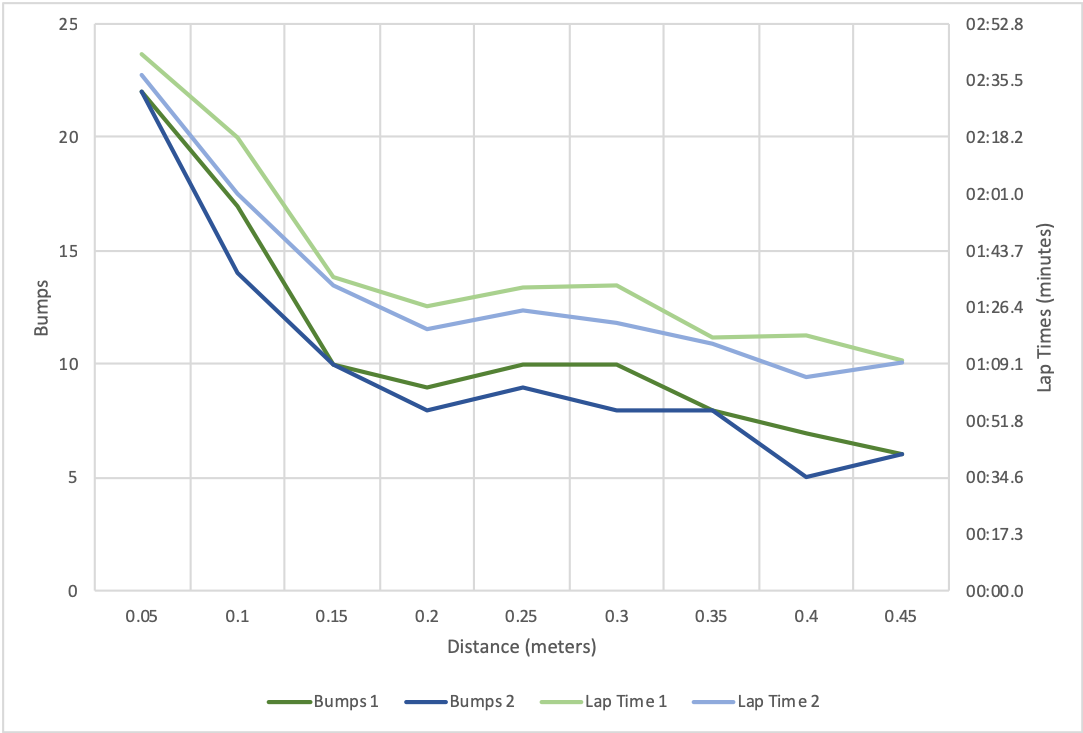
\includegraphics[width=\linewidth]{figures/results_graph.png}
\caption{Results graph}
  \label{fig:graph-results}
\end{figure}

\begin{comment}
Todo:
\begin{itemize}
    \item state that results are in line with the hypothesis
    \item place results in table
    \item provide link to youtube video
\end{itemize}
\end{comment}

% ----------------------------------------------------------------------------

\section{Discussion}

\begin{comment}
Todo:
\begin{itemize}
    \item suggest improvements (better quality sensors with less noise? more sensors?)
    \item make arena as consistent as possible (obstacles, wall placement, lighting)
\end{itemize}
\end{comment}

% ----------------------------------------------------------------------------

\section{Conclusion}

\begin{comment}
Todo:
\begin{itemize}
    \item single paragraph
    \item what this research set out to do and the results of the research
\end{itemize}
\end{comment}

% ----------------------------------------------------------------------------

\clearpage
\bibliographystyle{plainnat}
\bibliography{bibliography}

\begin{appendices}
\section{Raw Results}
\begin{table}[ht]
\begin{tabular}{l|l|l|l|l|}
\cline{2-5}
                                        & \multicolumn{2}{c|}{\textbf{Trial 1}}                & \multicolumn{2}{c|}{\textbf{Trial 2}}                \\ \hline
\multicolumn{1}{|l|}{\textbf{Distance}} & \textit{\textbf{Bumps}} & \textit{\textbf{Lap Time}} & \textit{\textbf{Bumps}} & \textit{\textbf{Lap Time}} \\ \hline
\multicolumn{1}{|l|}{\textbf{0.05}}     & 22                      & 02:43.8                    & 22                      & 02:37.0                    \\ \hline
\multicolumn{1}{|l|}{\textbf{0.1}}      & 17                      & 02:18.0                    & 14                      & 02:01.0                    \\ \hline
\multicolumn{1}{|l|}{\textbf{0.15}}     & 10                      & 01:35.7                    & 10                      & 01:33.3                    \\ \hline
\multicolumn{1}{|l|}{\textbf{0.2}}      & 9                       & 01:26.6                    & 8                       & 01:19.6                    \\ \hline
\multicolumn{1}{|l|}{\textbf{0.25}}     & 10                      & 01:32.0                    & 9                       & 01:25.0                    \\ \hline
\multicolumn{1}{|l|}{\textbf{0.3}}      & 10                      & 01:33.3                    & 8                       & 01:22.0                    \\ \hline
\multicolumn{1}{|l|}{\textbf{0.35}}     & 8                       & 01:17.5                    & 8                       & 01:15.6                    \\ \hline
\multicolumn{1}{|l|}{\textbf{0.4}}      & 7                       & 01:17.8                    & 5                       & 01:05.0                    \\ \hline
\multicolumn{1}{|l|}{\textbf{0.45}}     & 6                       & 01:10.3                    & 6                       & 01:09.9                    \\ \hline
\end{tabular}
\end{table}

\end{appendices}

\end{document}